%%
%% This is file `sample-sigconf.tex',
%% generated with the docstrip utility.
%%
%% The original source files were:
%%
%% samples.dtx  (with options: `sigconf')
%% 
%% IMPORTANT NOTICE:
%% 
%% For the copyright see the source file.
%% 
%% Any modified versions of this file must be renamed
%% with new filenames distinct from sample-sigconf.tex.
%% 
%% For distribution of the original source see the terms
%% for copying and modification in the file samples.dtx.
%% 
%% This generated file may be distributed as long as the
%% original source files, as listed above, are part of the
%% same distribution. (The sources need not necessarily be
%% in the same archive or directory.)
%%
%%
%% Commands for TeXCount
%TC:macro \cite [option:text,text]
%TC:macro \citep [option:text,text]
%TC:macro \citet [option:text,text]
%TC:envir table 0 1
%TC:envir table* 0 1
%TC:envir tabular [ignore] word
%TC:envir displaymath 0 word
%TC:envir math 0 word
%TC:envir comment 0 0
%%
%%
%% The first command in your LaTeX source must be the \documentclass
%% command.
%%
%% For submission and review of your manuscript please change the
%% command to \documentclass[manuscript, screen, review]{acmart}.
%%
%% When submitting camera ready or to TAPS, please change the command
%% to \documentclass[sigconf]{acmart} or whichever template is required
%% for your publication.
%%
%%
\documentclass[sigconf]{acmart}

\usepackage{bm}
\usepackage{algorithm}
\usepackage[noEnd=True]{algpseudocodex}
\usepackage{tikz}
\usepackage{listings}
\usepackage{float}
\floatstyle{plain}
\newfloat{Figure}{t}{myc}

\definecolor{dkgreen}{rgb}{0,0.6,0}
\definecolor{gray}{rgb}{0.5,0.5,0.5}
\definecolor{mauve}{rgb}{0.58,0,0.82}
\definecolor{verylightgray}{rgb}{.97,.97,.97}

\lstset{frame=tb,
  language=Python,
  aboveskip=3mm,
  belowskip=3mm,
  showstringspaces=false,
  columns=flexible,
  basicstyle={\small\ttfamily},
  numbers=none,
  backgroundcolor = \color{verylightgray},
  numberstyle=\tiny\color{gray},
  keywordstyle=\color{blue},
  commentstyle=\color{black},
  stringstyle=\color{black},
  breaklines=true,
  breakautoindent=false,
  breakindent=0pt,
  breakatwhitespace=true,
  tabsize=3
}

\usepackage{pgfplots}
\pgfplotsset{
    width=8cm,
    compat=1.9,
    legend style={
      fill,
      at={(0.50,-0.35)},
      legend columns=1,
      legend cell align=left,
      anchor=north
      }
    }
%%
%% \BibTeX command to typeset BibTeX logo in the docs
\AtBeginDocument{%
  \providecommand\BibTeX{{%
    Bib\TeX}}}

%% Rights management information.  This information is sent to you
%% when you complete the rights form.  These commands have SAMPLE
%% values in them; it is your responsibility as an author to replace
%% the commands and values with those provided to you when you
%% complete the rights form.
\setcopyright{acmlicensed}
\copyrightyear{2018}
\acmYear{2018}
\acmDOI{XXXXXXX.XXXXXXX}

%% These commands are for a PROCEEDINGS abstract or paper.
\acmConference[Conference acronym 'XX]{Make sure to enter the correct
  conference title from your rights confirmation emai}{June 03--05,
  2018}{Woodstock, NY}
%%
%%  Uncomment \acmBooktitle if the title of the proceedings is different
%%  from ``Proceedings of ...''!
%%
%%\acmBooktitle{Woodstock '18: ACM Symposium on Neural Gaze Detection,
%%  June 03--05, 2018, Woodstock, NY}
\acmISBN{978-1-4503-XXXX-X/18/06}


%%
%% Submission ID.
%% Use this when submitting an article to a sponsored event. You'll
%% receive a unique submission ID from the organizers
%% of the event, and this ID should be used as the parameter to this command.
%%\acmSubmissionID{123-A56-BU3}

%%
%% For managing citations, it is recommended to use bibliography
%% files in BibTeX format.
%%
%% You can then either use BibTeX with the ACM-Reference-Format style,
%% or BibLaTeX with the acmnumeric or acmauthoryear sytles, that include
%% support for advanced citation of software artefact from the
%% biblatex-software package, also separately available on CTAN.
%%
%% Look at the sample-*-biblatex.tex files for templates showcasing
%% the biblatex styles.
%%

%%
%% The majority of ACM publications use numbered citations and
%% references.  The command \citestyle{authoryear} switches to the
%% "author year" style.
%%
%% If you are preparing content for an event
%% sponsored by ACM SIGGRAPH, you must use the "author year" style of
%% citations and references.
%% Uncommenting
%% the next command will enable that style.
%%\citestyle{acmauthoryear}


%%
%% end of the preamble, start of the body of the document source.
\begin{document}

%%
%% The "title" command has an optional parameter,
%% allowing the author to define a "short title" to be used in page headers.
\title{CiteQ: Analysis on Citation Purposes: University of Waterloo Computer Science Faculty Case Study} 

%%
%% The "author" command and its associated commands are used to define
%% the authors and their affiliations.
%% Of note is the shared affiliation of the first two authors, and the
%% "authornote" and "authornotemark" commands
%% used to denote shared contribution to the research.
\author{Onur Eren Arpaci}
\email{oearpaci@uwaterloo.ca}
\affiliation{%
  \institution{University of Waterloo}
  \streetaddress{200 University Ave W}
  \city{Waterloo}
  \state{Ontario}
  \country{Canada}
  \postcode{N2L 3G1}
}

%%
%% By default, the full list of authors will be used in the page
%% headers. Often, this list is too long, and will overlap
%% other information printed in the page headers. This command allows
%% the author to define a more concise list
%% of authors' names for this purpose.
\renewcommand{\shortauthors}{Arpaci}

%%
%% The abstract is a short summary of the work to be presented in the
%% article.
\begin{abstract}
  TODO: Write abstract
\end{abstract}

%%
%% The code below is generated by the tool at http://dl.acm.org/ccs.cfm.
%% Please copy and paste the code instead of the example below.
%%
\begin{CCSXML}
    <ccs2012>
       <concept>
           <concept_id>10002951.10003317</concept_id>
           <concept_desc>Information systems~Information retrieval</concept_desc>
           <concept_significance>300</concept_significance>
           </concept>
       <concept>
           <concept_id>10002944.10011123.10011131</concept_id>
           <concept_desc>General and reference~Experimentation</concept_desc>
           <concept_significance>500</concept_significance>
           </concept>
       <concept>
           <concept_id>10003456.10010927.10003619</concept_id>
           <concept_desc>Social and professional topics~Cultural characteristics</concept_desc>
           <concept_significance>100</concept_significance>
           </concept>
     </ccs2012>
\end{CCSXML}
    
\ccsdesc[300]{Information systems~Information retrieval}
\ccsdesc[500]{General and reference~Experimentation}
\ccsdesc[100]{Social and professional topics~Cultural characteristics}

%%
%% Keywords. The author(s) should pick words that accurately describe
%% the work being presented. Separate the keywords with commas.
\keywords{Citation Purpose, Citation Analysis, Citation Trends, LLM classification}
%% A "teaser" image appears between the author and affiliation
%% information and the body of the document, and typically spans the
%% page.

\received{20 February 2007}
\received[revised]{12 March 2009}
\received[accepted]{5 June 2009}

%%
%% This command processes the author and affiliation and title
%% information and builds the first part of the formatted document.
\maketitle

\section{Introduction}
The predominant and widely recognized scientometric indicator is the number 
of citations a paper garners. Nevertheless, it's crucial to acknowledge that 
papers can be cited for diverse reasons. A citation may stem from a paper 
serving as the foundational work for current research, acting as a competitor 
in the field, or being subject to critique. 

The purpose of this paper is to study the citation purposes and its affects
on other scientometric indicators. We aim to answer the following research 
questions:

\begin{enumerate}
    \item[RQ1] Do the citation purposes affect the total number of
    citations a paper or a researcher receives? (i.e. is there a karma effect?)
    \item[RQ2] How does the distribution of citation purposes change over time?
    \item[RQ3] Is there any difference in the distribution of citation purposes
    between same institution researchers and different institution researchers? 
    \item[RQ4] How does the distribution of citation purposes change over the
    duration of a researcher's career?
\end{enumerate}

To answer these questions, we collected the publication and citation data of
the University of Waterloo Computer Science faculty members. We then used
the large language model (LLM) llama2 \cite{touvron2023llama} to classify the citation 
purposes of each paper. We then analyzed this data to answer the research questions.

\section{Related Work}
Our work is related to a large body of research on citation analysis. Abu-Jbara et. al. \cite{abu2013purpose} provides a good starting point for citation purpose analysis. They propose 6 classes of citation purposes: criticizing, comparison, use, substantiating, basis, and neutral. We use these classes as the basis for our analysis.

\section{Methodology}
\subsection{Data Collection}
We used the Semantic Scholar (SS) API to collect the publication and citation data of all current (as of this writing) members of the University of Waterloo Computer Science faculty members. SS provides an API endpoint to retrieve the context of a citation. We used this endpoint to retrieve the citation context of each citation
made by a faculty member or to a faculty member. In total we collected data about 96 faculty members, 9,438 papers, and 697,609 citations. We formed an SQLite database, with the scheme shown in Figure \ref{fig:citeq-scheme}, to facilitate flexible querying of the data.

\begin{figure}[h]
    \centering
    \includegraphics[width=\linewidth]{citeq-scheme.png}
    \caption{CiteQ database scheme}
    \label{fig:citeq-scheme}
\end{figure}

\subsection{Citation Purpose Classification}
We experimented with a number of LLMs including chatGPT-3.5 \cite{brown2020language}, chatGPT-4.5 \cite{openai2023gpt4}, mistral \cite{jiang2023mistral}, and llama2 \cite{touvron2023llama}. Although chatGPT models performed slightly better in terms of accuracy, we decided to use llama2 with 7 billion parameters due to its low cost. We used 5 RTX4090 GPUs for 10 hours to classify the citation purposes of all 697,609 citations.

We used the following citation purpose classes: criticizing, comparison, use, substantiating, basis, and neutral. The Figure \ref{figure:prompt-template} shows the prompt template we used.

\subsubsection{Evaluation}
We hand labeled 100 citations to evaluate the accuracy of the classification.
The results are shown in Table \ref{table:evaluation}. We achieved an accuracy of 0.82. The accuracy of the classification is not as high as we would like. However, we believe that it is sufficient for our purposes.

\begin{table}[h]
    \centering
    \begin{tabular}{|l|l|l|l|l|}
        \hline
        \textbf{Class/Model} & \textbf{llama2} & \textbf{mistral} & \textbf{GPT-3.5} & \textbf{GPT-4.5} \\ \hline
        Criticizing & 0.75 & 0.75 & 0.75 & 0.75 \\ \hline
        Comparison & 0.75 & 0.75 & 0.75 & 0.75 \\ \hline
        Use & 0.75 & 0.75 & 0.75 & 0.75 \\ \hline
        Substantiating & 0.75 & 0.75 & 0.75 & 0.75 \\ \hline
        Basis & 0.75 & 0.75 & 0.75 & 0.75 \\ \hline
        Neutral & 0.75 & 0.75 & 0.75 & 0.75 \\ \hline
        \textbf{Average} & \textbf{0.82} & \textbf{0.82} & \textbf{0.82} & \textbf{0.82} \\ \hline
    \end{tabular}
    \caption{Precision of different LLMs in citation purpose classification}
    \label{table:evaluation}
\end{table}

\begin{figure}
\begin{lstlisting}
"""
The following is a set of citation purpose categories, each category name is followed by a description of the category and an example of a sentence that belongs to this category.

Name: Criticizing
Description: Criticism can be positive or negative. A citing sentence is classified as "criticizing" when it mentions the weakness/strengths of the cited approach, negatively/positively criticizes the cited approach, negatively/positively evaluates the cited source.
Example: Chiang (2005) introduced a constituent feature to reward phrases that match a syntactic tree but did not yield significant improvement.

Name: Comparison
Description: A citing sentence is classified as "comparison" when it compares or contrasts the work in the cited paper to the author's work. It overlaps with the first category when the citing sentence says one approach is not as good as the other approach. In this case we use the first category.
Example: Our approach permits an alternative to minimum error-rate training (MERT; Och, 2003);

Name: Use
Description: A citing sentence is classified as "use" when the citing paper uses the method, idea or tool of the cited paper.
Example: We perform the MERT training (Och, 2003) to tune the optimal feature weights on the development set.

Name: Substantiating
Description: A citing sentence is classified as "substantiating" when the results, claims of the citing work substantiate, verify the cited paper and support each other.
Example: It was found to produce automated scores, which strongly correlate with human judgements about translation fluency (Papineni et al. , 2002).

Name: Basis
Description: A citing sentence is classified as "basis" when the author uses the cited work as starting point or motivation and extends on the cited work.
Example: Our model is derived from the hidden-markov model for word alignment (Vogel et al., 1996; Och and Ney, 2000).

Name: Neutral (Other)
Description: A citing sentence is classified as "neutral" when it is a neutral description of the cited work or if it doesn't come under any of the above categories.
Example: The solutions of these problems depend heavily on the quality of the word alignment (Och and Ney, 2000).

Classify the following in text citation into one of these categories. Only use a single category for each citation. Respond with only a single word, the name of the category.

{Citation Context}
"""
\end{lstlisting}
\caption{Prompt template used for citation purpose classification}
\label{figure:prompt-template}
\end{figure}

\section{Results}
Initial results

\begin{Figure}
  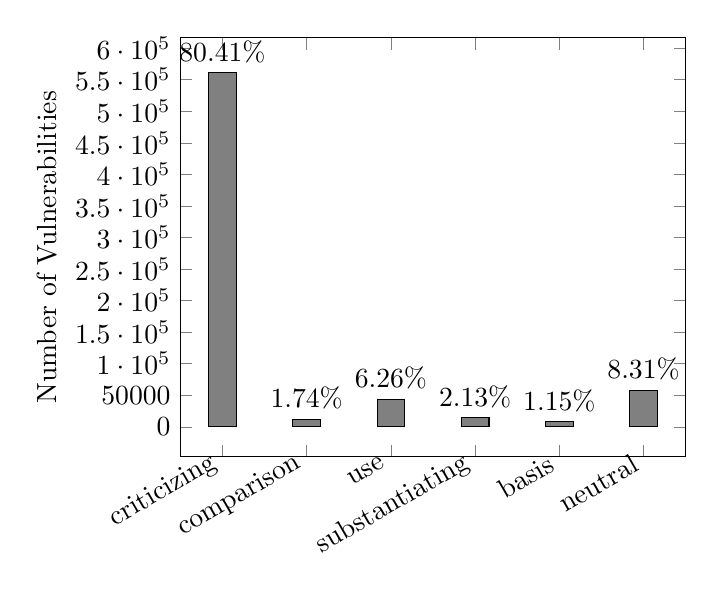
\begin{tikzpicture}
  \begin{axis}[
      symbolic x 
      coords={criticizing, comparison, use, substantiating, basis, neutral},
      scaled ticks=false,
      style={/pgf/number format/1000 sep=},
      xtick=data,
      xticklabel style = {rotate=30,anchor=east},
      ytick distance=50000,
      ylabel=Number of Vulnerabilities,
      point meta={(y/697609)*100},
      nodes near coords={\pgfmathprintnumber\pgfplotspointmeta\%}]
      \addplot[ybar,fill=gray] coordinates {
          (criticizing, 560986)
          (comparison, 12122)
          (use,43646)
          (substantiating, 14860)
          (basis, 8057)
          (neutral, 57938)
      };
  \end{axis}
  \end{tikzpicture}
  \caption{Distribution of Vulnerabilities }
  \label{graph:1}
  \end{Figure}

%%
%% The acknowledgments section is defined using the "acks" environment
%% (and NOT an unnumbered section). This ensures the proper
%% identification of the section in the article metadata, and the
%% consistent spelling of the heading.
% \begin{acks}
% To Robert, for the bagels and explaining CMYK and color spaces.
% \end{acks}

%%
%% The next two lines define the bibliography style to be used, and
%% the bibliography file.
\bibliographystyle{ACM-Reference-Format}
\bibliography{sample-base}


%%
%% If your work has an appendix, this is the place to put it.

\end{document}
\endinput
%%
%% End of file `sample-sigconf.tex'.
